\chapter{Ship design}
\head{This chaper describes the design considerations that has been thought of whilst designing a about 1 metre boat for this project.}

\section{LLI electronics}
The \ac{LLI} electronics should be a kind of plug and play device that can be put into serval smaller ship designs. It should provide outputs to control different kind of actuators, and it should also provide basic sensor readings to the \ac{HLI} and \ac{GRS}, whilst being able to have a few general IO pins to miscellaneous stuff.

The \ac{LLI} has been designed to allow for the mentioned functionality. As described in section~\vref{sec:platform} the \ac{LLI} is an embedded platform. In this case a Atmel AVR microcontroller has been choosen. The electronics/hardware used in this case is an Arduino Mega 2560, where a shield to interface all peripehals has been designed. The schematic for this can be seen in appendix~\vref{chap:schema}.

It has been designed as a box with the following features:
\begin{description}
\item[Serial]\hfill \\ interface supposed to be used to the \ac{HLI} with a baud rate of 115200 bps
\item[PWM]\hfill \\ outputs for actuators. Both some PWM outputs supposed to be used with servos and \ac{ESC}'s used in RC hobby, together with some full range and kilo hertz range frequencies, which could be used for modulating H-bridge drivers directly.
\item[I$^2$C]\hfill \\ option for aux communication \todo{hmm, maybe I actually forgot to wire this to the interface connector}
\item[Analog]\hfill \\ inputs which could be used for i.e. temperature sensors.
\item[Relay driver]\hfill \\ output, i.e. to cutoff actuator power.
\item[5V]\hfill \\ regulated output.
\end{description}

\begin{figure}
\centering
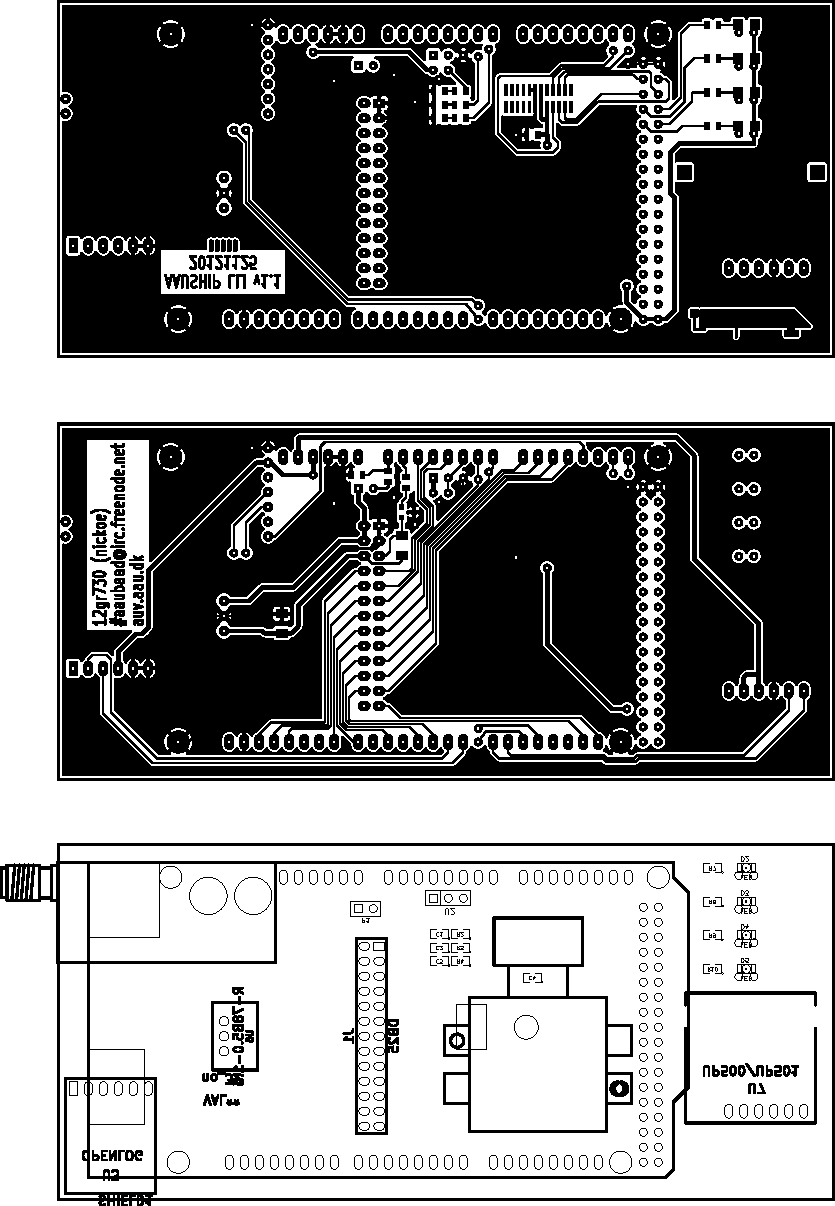
\includegraphics{img/lli-hw}
\label{fig:lli-hw}
\caption{Hardware layout for the LLI}
\end{figure}

\section{Bow thruster}
The ship design includes a bow thruster, which can be used to perform precision maneuvers in tight spaces. This component is not currently included in our control algorithms, because it has little or no effect on the ship when used at speeds above \todo{what speeds?}. It will be controlled by the \ac{LLI} with a direction and a \ac{PWM} signal. 

The electronic design of the bow thruster controller can be found in subsection \ref{subsec:bow thruster controller}: Bow thruster controller.
